%%%%%%%%%%%%%%%%%%%%%%%%%%%%%%%%%%%%%%%%%%%%%%%
\chapter{Introduction and Motivation} \label{chap:introduction}
%%%%%%%%%%%%%%%%%%%%%%%%%%%%%%%%%%%%%%%%%%%%%%%

In 1948, scientists at the Bell Laboratories achieved two landmark research results:
Claude E.~Shannon published his paper \emph{A mathematical theory of communication} and John Bardeen, Walter Brattain and William Shockley announced the invention of the \emph{transistor effect}.

\cite{Arikan}

A binomial distribution is shown in Figure~\ref{fig:coin_bino}.

%\begin{figure}[!htb]
%    \centering
%    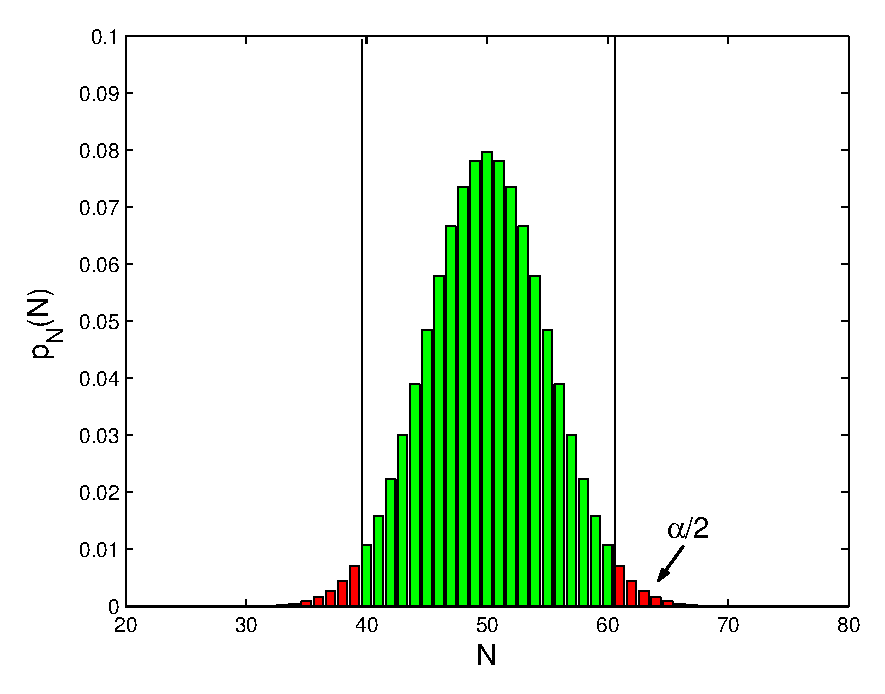
\includegraphics[width=0.8\textwidth]{./figures/coin_bino.eps}
%    \caption{PDF $p_N(N)$ of the number N of times that the head side is up.}
%    \label{fig:coin_bino}
%\end{figure}

For further information, the reader is referred to~\cite{Cover}.\newline

Traditionally FEC chains are developed in hardware i.e FPGA’s or ASIC’s to achieve low latency and high throughput.
Development in FPGA/hardware requires more time and costly.
With recent advances in General Purpose Processors it is possible to achieve required latency and throughput with software implementations without custom hardware.
Software implementations are flexible and easy to maintain compared hardware implementations.

However algorithms need to be adopted/optimized to efficiently implement in software.

Recent advances in the modern processors such as SIMD units can be utilized to achieve low latency and high throughput.

\cite{PolarCodesPrimaryConcepts}

\cite{DesignOfPolarCodes5G}

\cite{fastSSC}

\cite{multiGbpsSoftwareDec}

\cite{SCL}

\clearpage
